\section{Free Independence from Combinatorics}
\paragraph{Definition.} Define $\t(X^{n_1}Y^{n_2}X^{n_3}\dots Y^{n_m})$ where $n_i > 0$ for $1 < i < m$ as follows:
\begin{enumerate}
    \item Let $n = \sum n_i$, and let $[n] = \{1, \dots, n\}$ denote a vertex set of $n$ points ordered clockwise on the unit circle.
    \item Color the first $n_1$ vertices green, the next vertices $n_2$ red, and so on, alternating between green and red.
    \item Let $\t(X^{n_1}Y^{n_2}X^{n_3}\dots Y^{n_m})$ be the number of simple undirected graphs on $[n]$ such that each edge is either red or green and
    \begin{itemize}
        \item A red edge only connectes red vertices (and same for green).
        \item Two opposite colored edges do not intersect.
    \end{itemize}
\end{enumerate}
We then extend $\t$ (which we will call ``trace'') linearly to formal sums of monomials, possibly multiplied by scalars.

\paragraph{Recursive Relations.} We would like to express $\t(X^{n_1}Y^{n_2}X^{n_3}\dots Y^{n_m})$ as a function of the traces of monomials of lower degrees.

To hopefully illuminate what is happening, we present a simple example. Suppose we want to compute $\t(XYXY)$. Let the hat superscript denote omission, i.e. $\t(X\hat{Y}XY) = \t(X^2Y)$. Then note:
\begin{figure}[H]
    \centering
    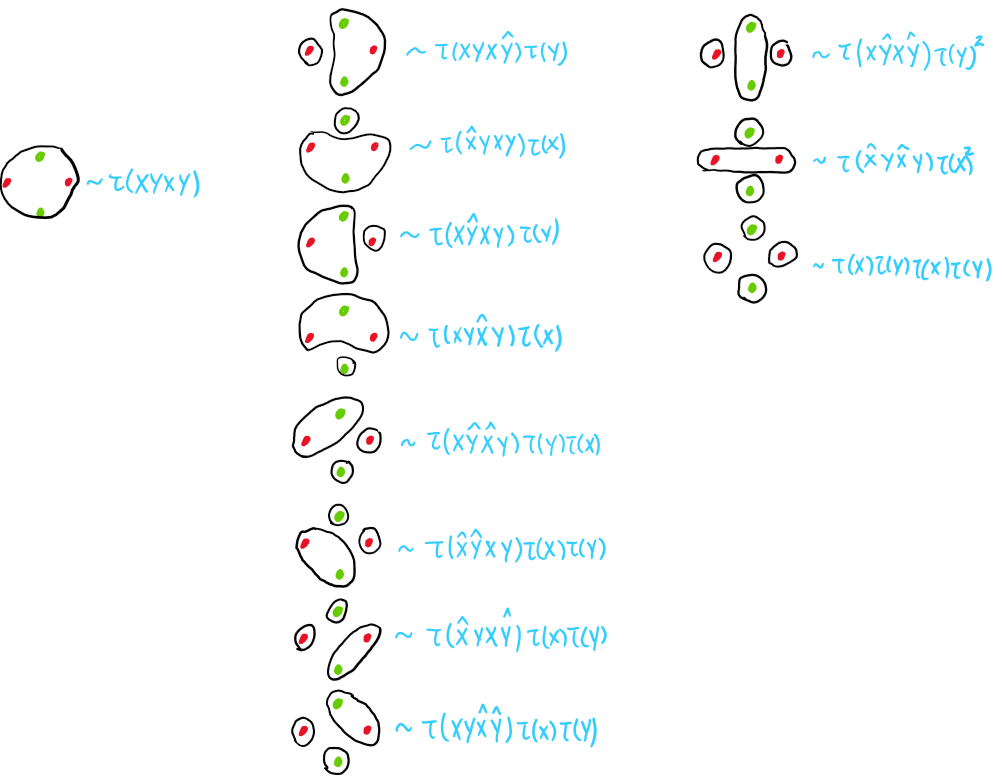
\includegraphics[width=0.9\linewidth]{figures/xyxy.png}
\end{figure}
By keeping track of the different ways a graph can be decomposed into non-crossing subgraphs, we can use inclusion-exclusion to conclude that
\[
    \begin{split}
        \t(XYXY) & = \sum_{i \in [4]} \t(\text{[omit $i$-th term]})\t(\text{[$i$-th term]})                             \\
                 & - \sum_{i,j \in [4]} \t(\text{[omit $i,j$-th term]})\t(\text{[$i$-th term]})\t(\text{[$j$-th term]}) \\
                 & + \sum_{i,j,k \in [4]} \t(X)\t(Y)\t(X)\t(Y)                                                          \\
                 & - \t(X)\t(Y)\t(X)\t(Y).
    \end{split}
\]
The same strategy works in general. By keeping track of how graphs can be decomposed into non-crossing subgraphs, is it not hard to apply inclusion-exclusion to see
\[
    \t(X^{n_1}Y^{n_2}X^{n_3}\dots Y^{n_m}) = \sum (-1)^{k-1}\t\left( \prod \cdots \right) \underbrace{\prod \t(\cdot)}_{\text{$k$ terms}}.
\]
[Notation is omitted as it is rather tedious.] After rearranging, the recursive relation becomes
\[
    \t\left( (X^{n_1} - \t(X^{n-1})) (Y^{n_2} - \t(Y^{n_2}))\dots (Y^{n_m} - \t(Y^{n_m})) \right) = 0.
\]
This is precisely the definition of free independence! Therefore:
\[
    \boxed{\text{Free indep. is a recursive relation of graphs derived by inclusion-exclusion.}}
\]
Indeed, knowing $\t(X)$ and $\t(Y)$, this recursive relation allows us to compute the trace of any monomial (and thus, any polynomial). Hence free independence completely characterizes $\t$.

\section{Passing to Cumulants}
\paragraph{Definition.} Define $\kappa(X^{n_1}Y^{n_2}X^{n_3}\dots Y^{n_m})$ where $n_i > 0$ for $1 < i < n_m$ as follows:
\begin{enumerate}
    \item Same as $\t$'s definition.
    \item Same as $\t$'s definition.
    \item Let $\kappa(X^{n_1}Y^{n_2}X^{n_3}\dots Y^{n_m})$ be the number of simple undirected \textbf{geometrically connected} graphs on $[n]$ such that each edge is either red or green and
    \begin{itemize}
        \item A red edge only connectes red vertices (and same for green).
        \item Two opposite colored edges do not intersect.
    \end{itemize}
\end{enumerate}
We then extend $\kappa$ linearly to formal sums of monomials, possibly multiplied by scalars.

\paragraph{Observations.} Note:
\begin{itemize}
    \item $\kappa\left( (X+Y)^n \right)$ = \# of graphs on $[n]$ for all colorings of the $n$ vertices.
    \item $\kappa\left( X^n \right)$ = \# of graphs on $[n]$ if all vertices are green.
    \item $\kappa\left( Y^n \right)$ = \# of graphs on $[n]$ if all vertices are red.
\end{itemize}
Furthermore, note that a geometrically connected graph with non-crossing colors on $[n]$ must have all vertices of the same color, so we conclude
\[
    \kappa\left( (X+Y)^n \right) = \kappa(X^n) + \kappa(Y^n).
\]

\section{Generalizing}
We now have seen two interesting equations:
\begin{equation}
    \label{free-ind}
    \t\left( (X^{n_1} - \t(X^{n-1})) (Y^{n_2} - \t(Y^{n_2}))\dots (Y^{n_m} - \t(Y^{n_m})) \right) = 0,
\end{equation}
\begin{equation}
    \label{cum-lin}
    \kappa\left( (X+Y)^n \right) = \kappa(X^n) + \kappa(Y^n).
\end{equation}
Because \ref{free-ind} completely determines $\t$ (given initial data), and $\kappa(X^n), \kappa(Y^n)$ can be recursively derived from $\t(X^n), \t(Y^n)$, we would expect that any $\t$ satisfying \ref{free-ind} will produce $\kappa$ satisfying \ref{cum-lin}. This is the driving principle behind why free cumulants linearize freely independent random variables.


%%% Local Variables:
%%% TeX-master: "main"
%%% End: